\chapter{System Design}
\section{Front-End Design}
Stuff about front-end...

Login Page See Figure ~\ref{image:loginPage}
\begin{figure}[h!]
    \caption{Login Page}
    \label{image:loginPage}
    \centering
    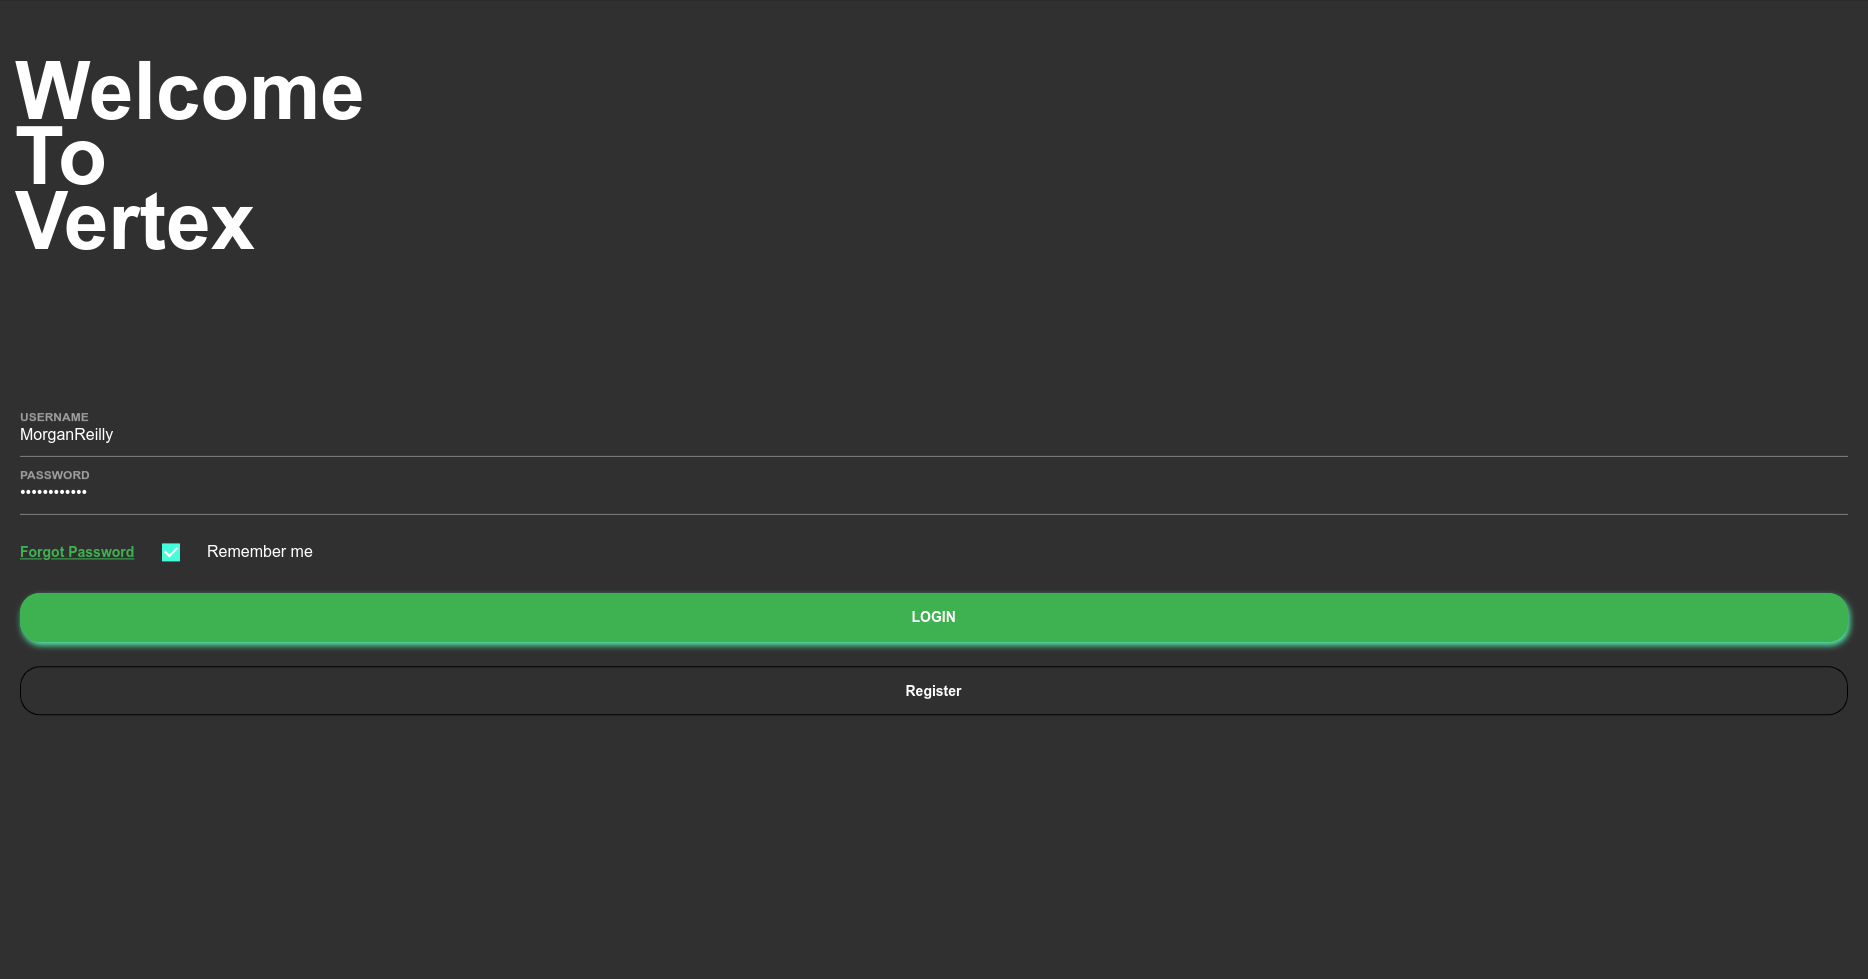
\includegraphics[width=0.7\textwidth]{images/pageScreenshots/loginPage.png}
\end{figure}

Register Page See Figure ~\ref{image:registerPage}
\begin{figure}[h!]
    \caption{Register Page}
    \label{image:registerPage}
    \centering
    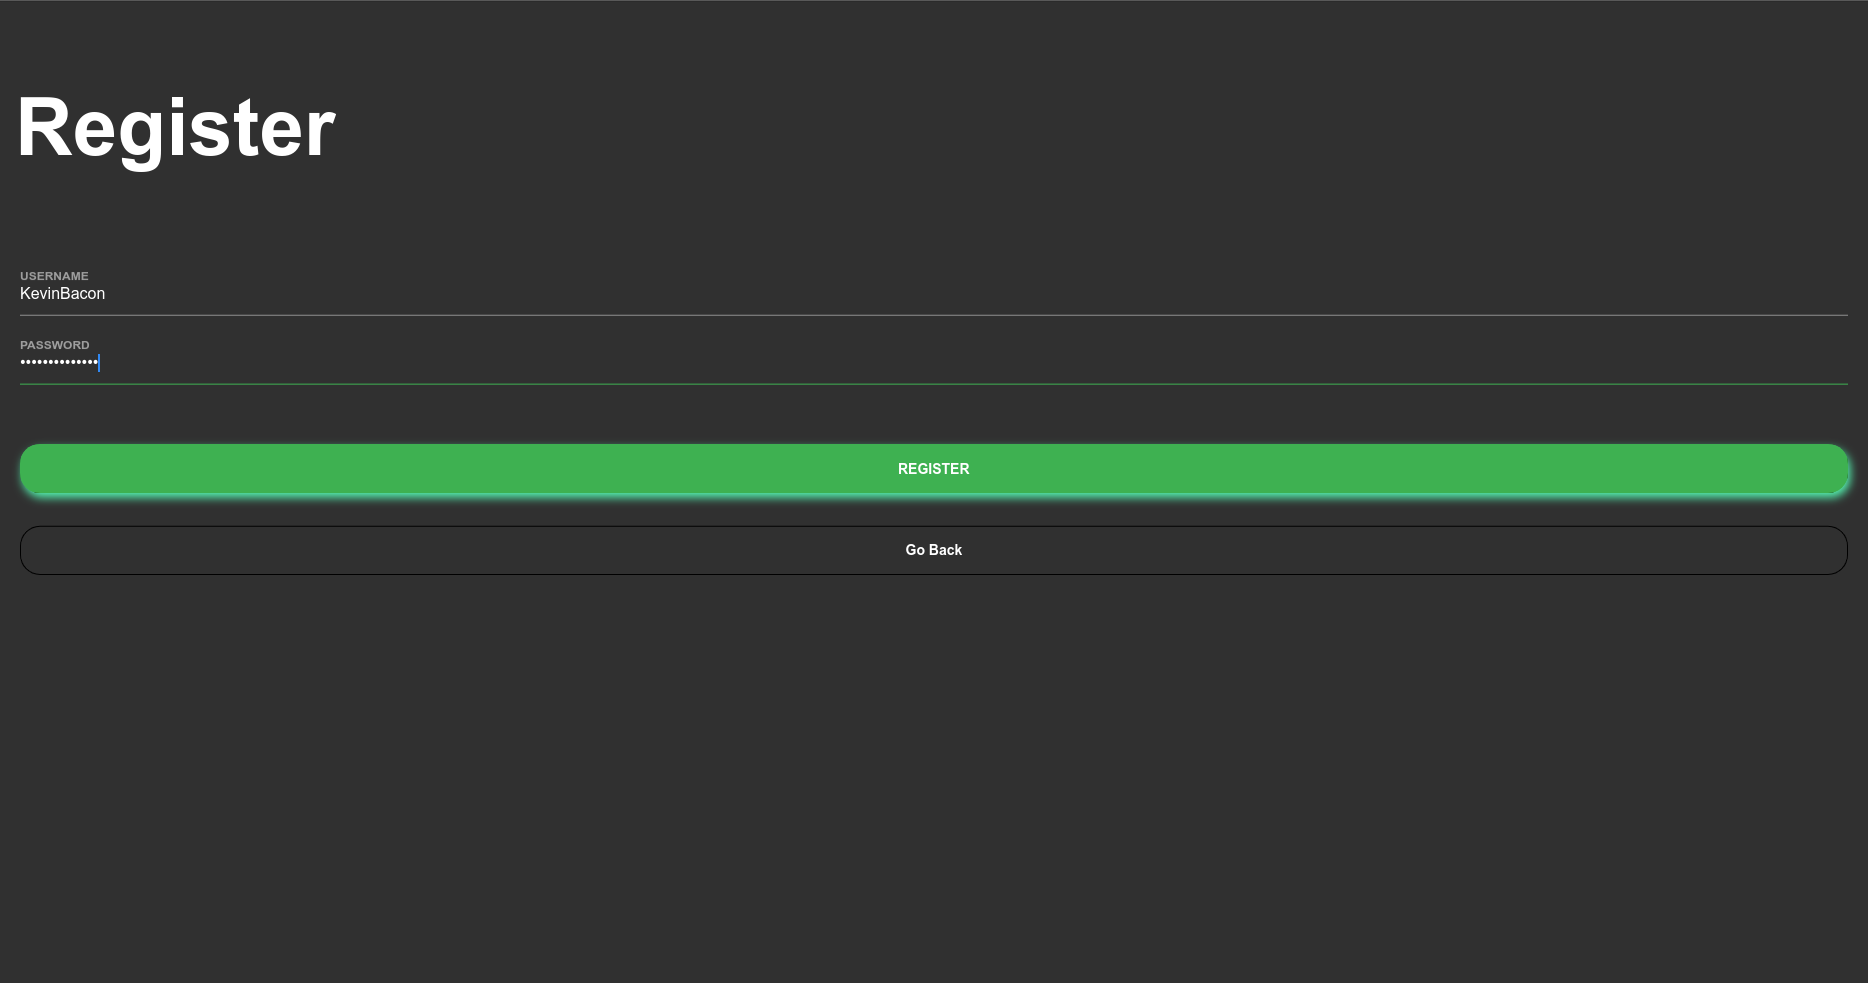
\includegraphics[width=0.7\textwidth]{images/pageScreenshots/registerPage.png}
\end{figure}

Home Page See Figure ~\ref{image:homePage}
\begin{figure}[h!]
    \caption{Home Page}
    \label{image:homePage}
    \centering
    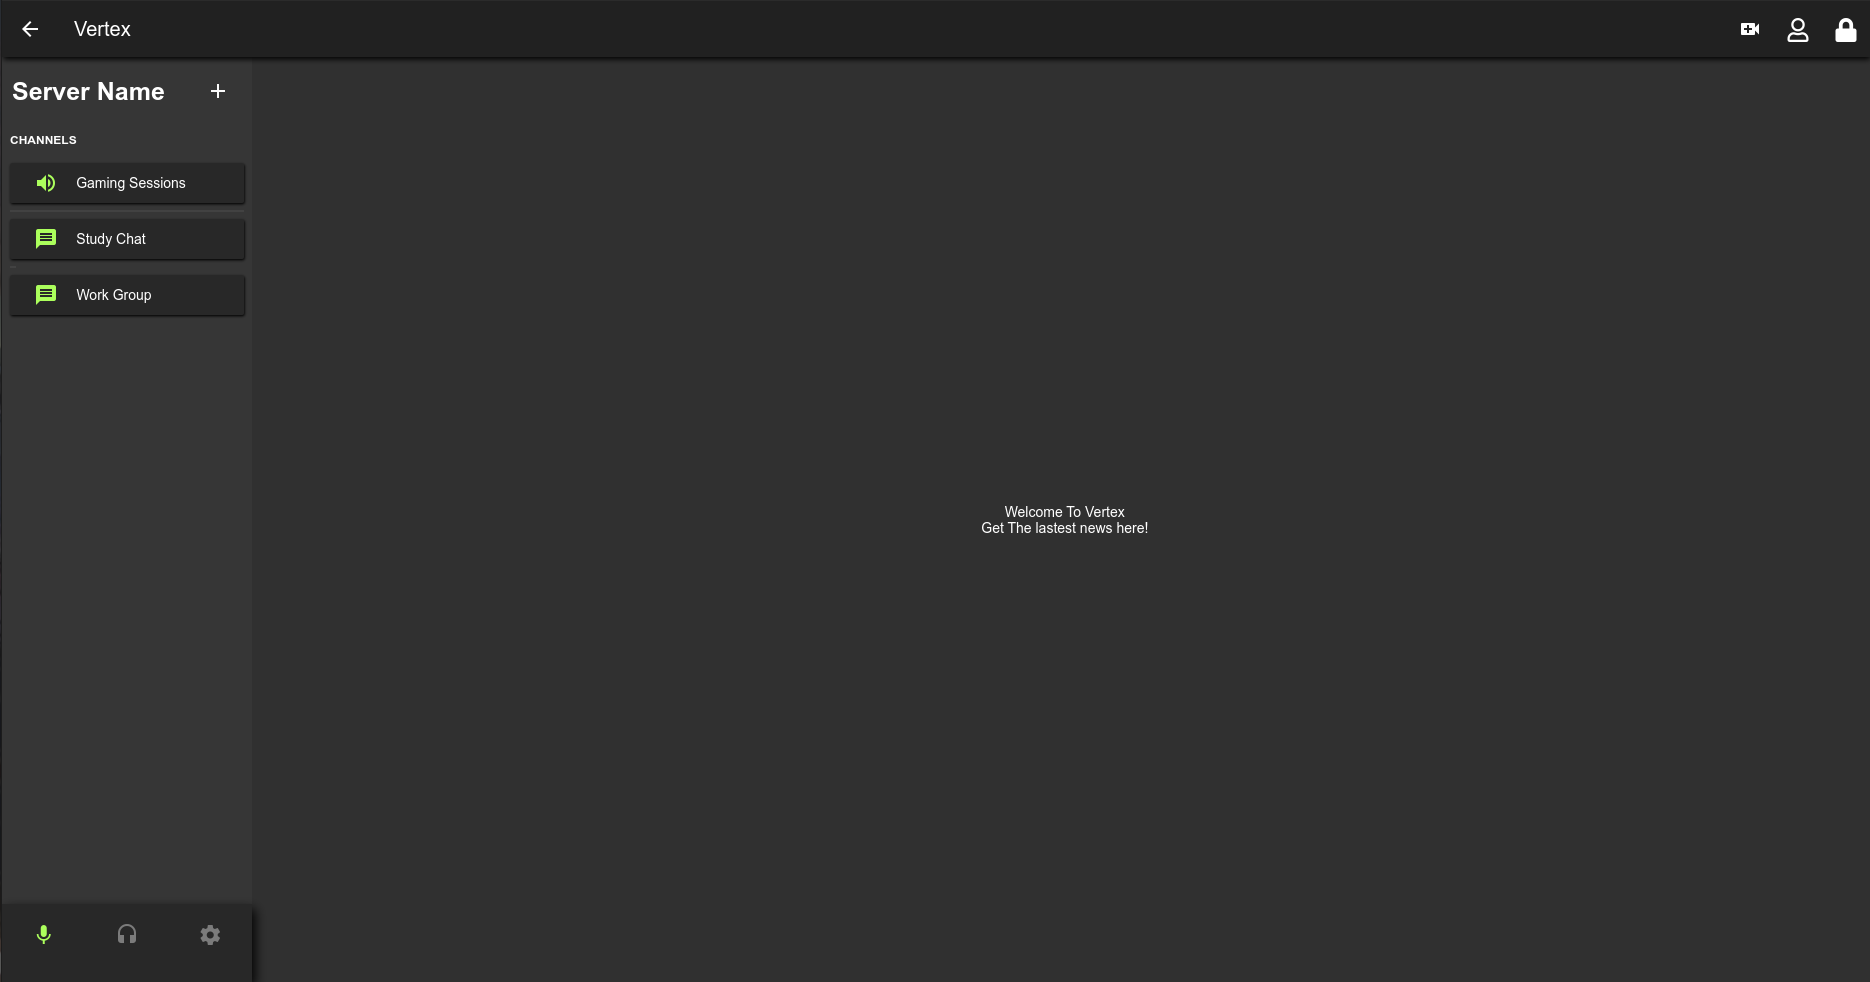
\includegraphics[width=0.7\textwidth]{images/pageScreenshots/homeScreen.png}
\end{figure}

Peer Connection Lobby See Figure ~\ref{image:peerConnectionLobby}
\begin{figure}[h!]
    \caption{Peer Connection Lobby}
    \label{image:peerConnectionLobby}
    \centering
    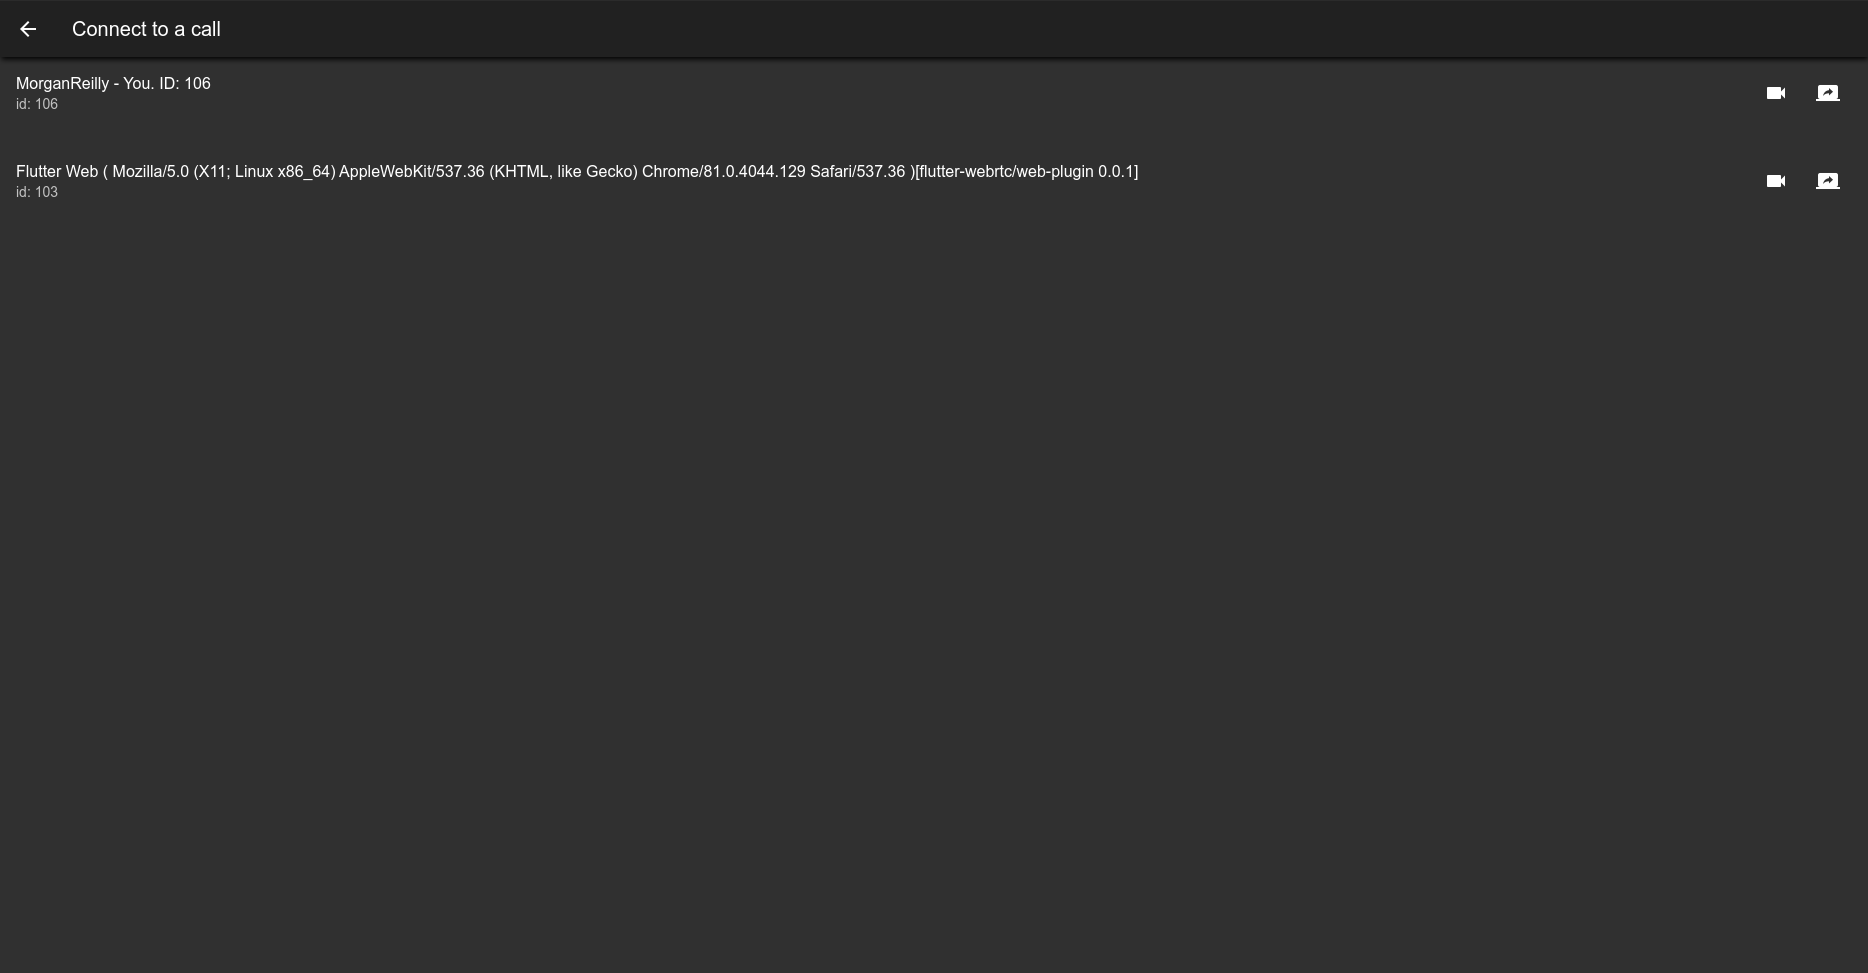
\includegraphics[width=0.7\textwidth]{images/pageScreenshots/callLobby.png}
\end{figure}

Successful WebRTC Functionality See Figure ~\ref{image:webRTCProof}
\begin{figure}[h!]
    \caption{Successful WebRTC Functionality}
    \label{image:webRTCProof}
    \centering
    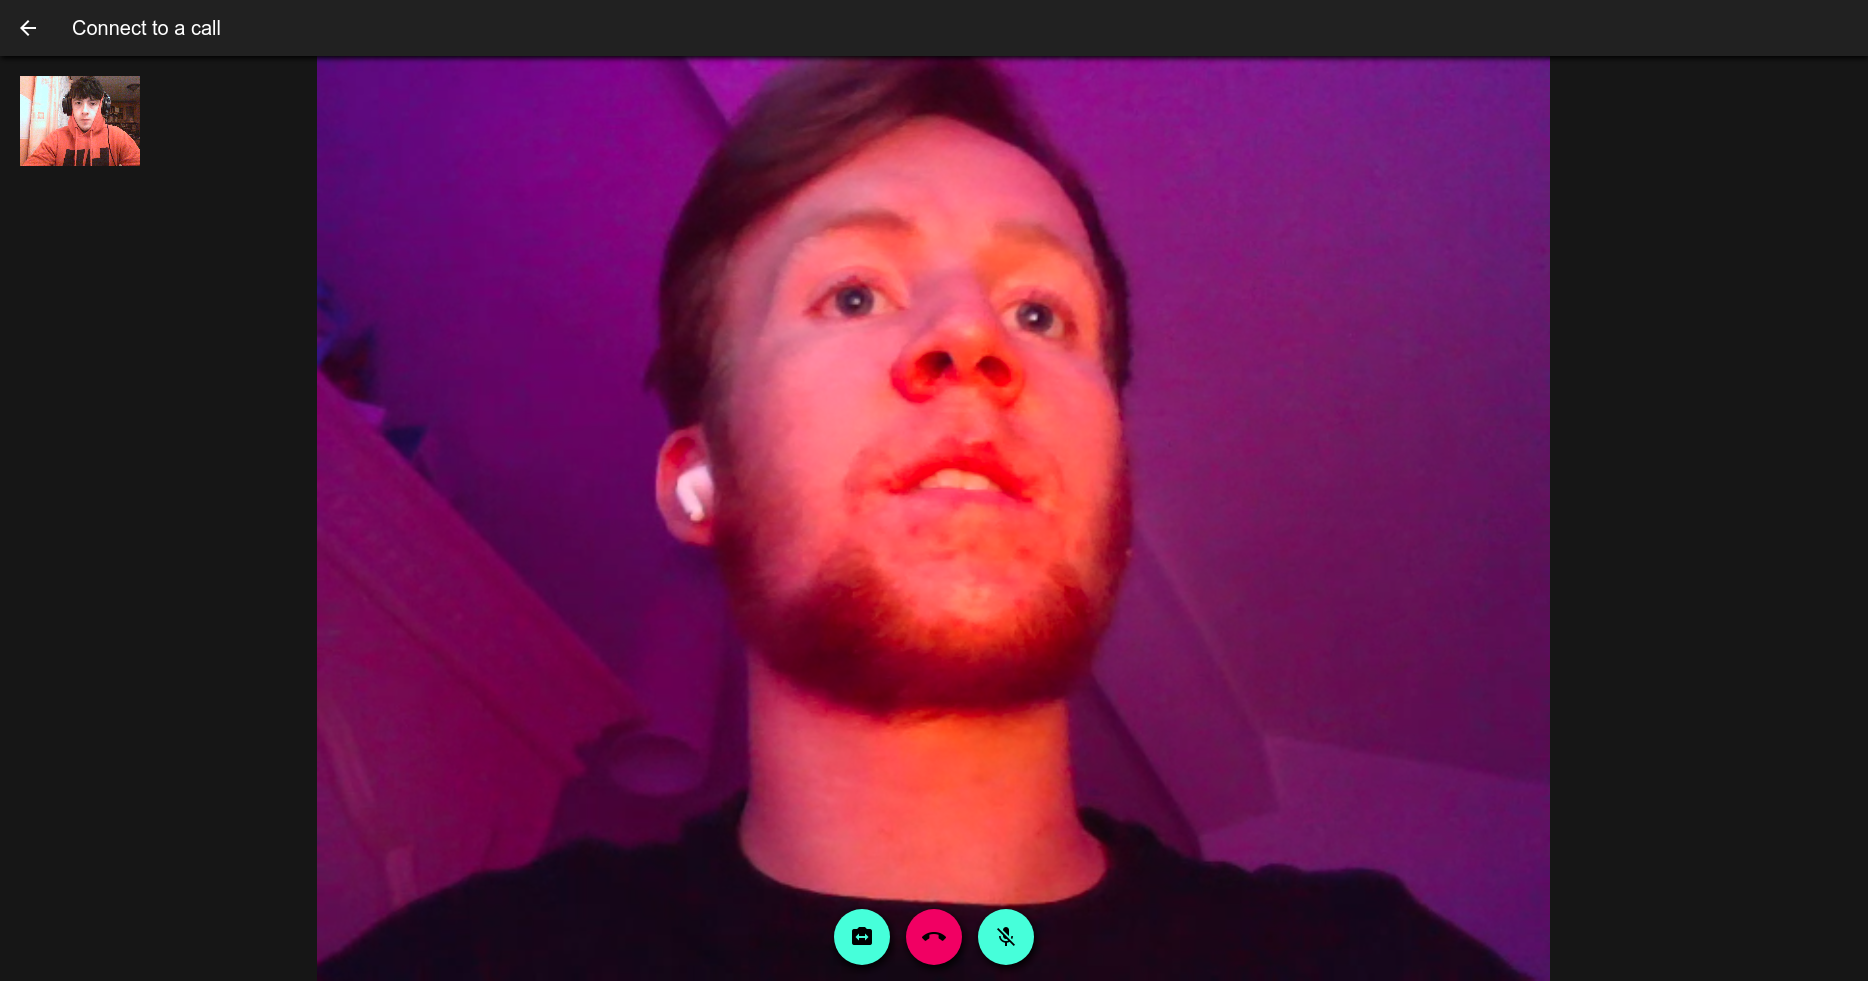
\includegraphics[width=0.7\textwidth]{images/pageScreenshots/webRTCProof.png}
\end{figure}

Channel Creation See Figure ~\ref{image:channelCreation}
\begin{figure}[h!]
    \caption{Channel Creation}
    \label{image:channelCreation}
    \centering
    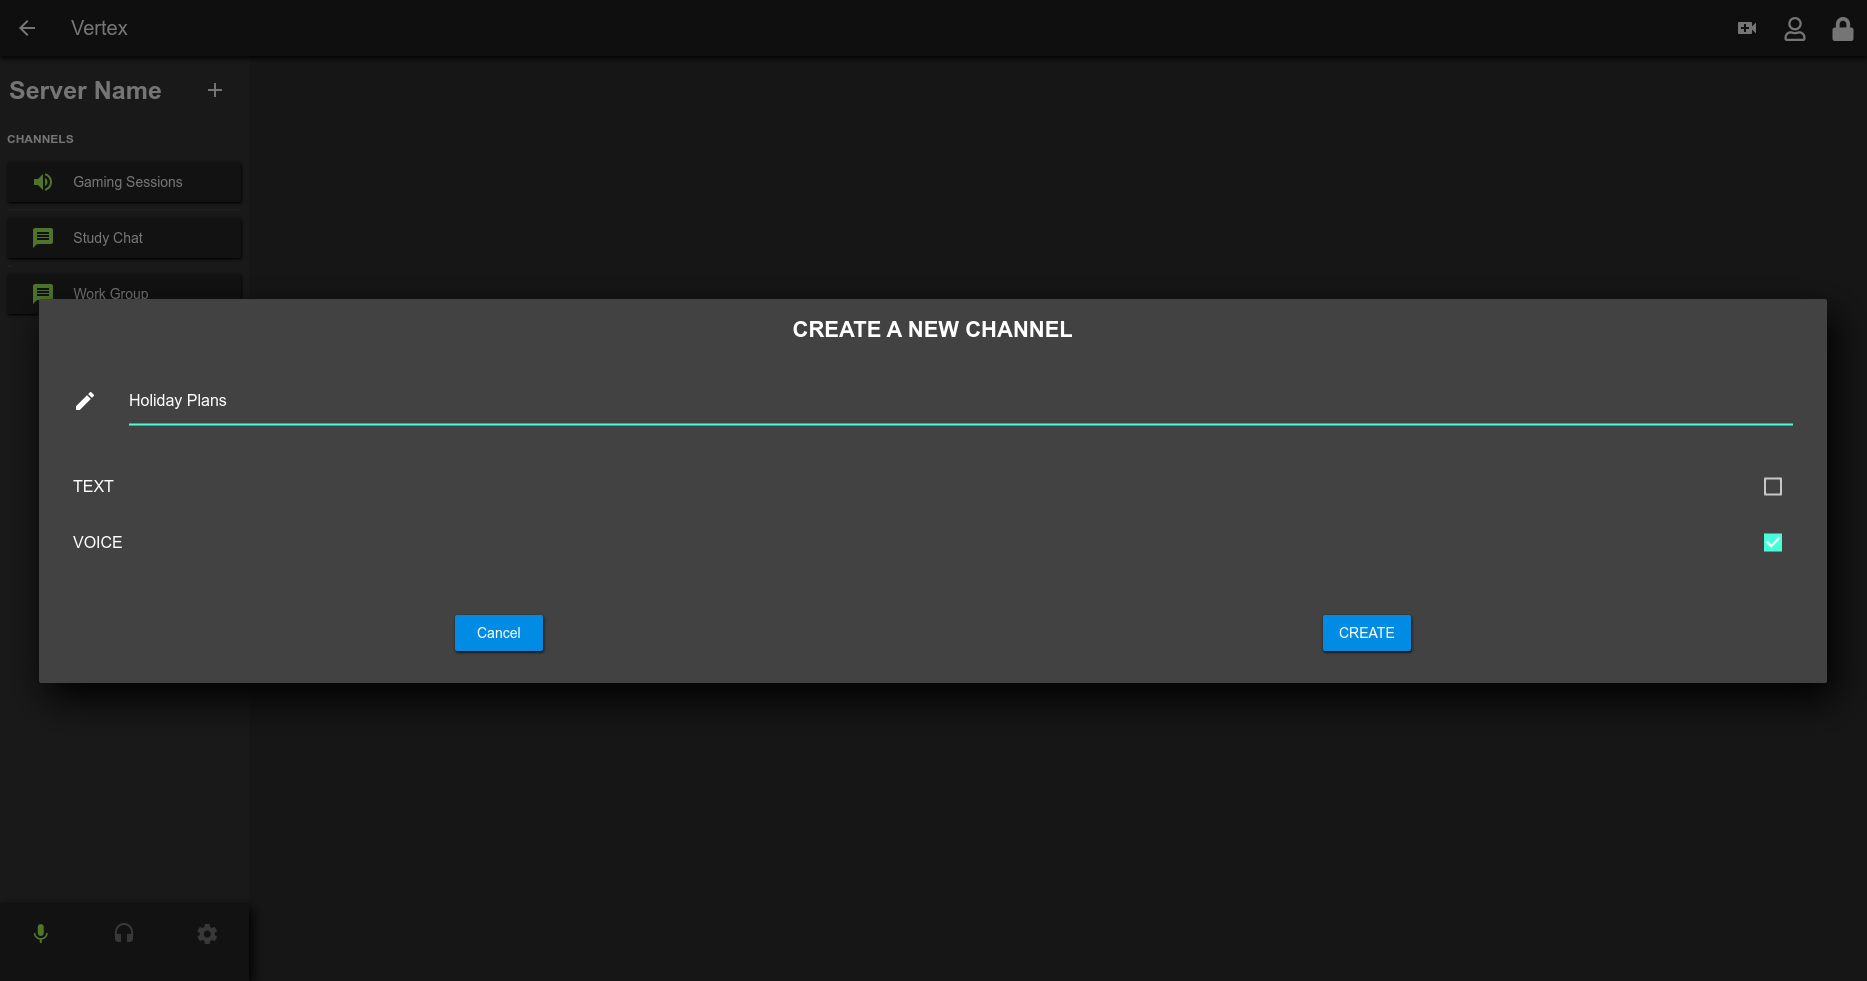
\includegraphics[width=0.7\textwidth]{images/pageScreenshots/channelCreation.png}
\end{figure}

Channel Deletion See Figure ~\ref{image:channelDeletion}
\begin{figure}[h!]
    \caption{Channel Deletion}
    \label{image:channelDeletion}
    \centering
    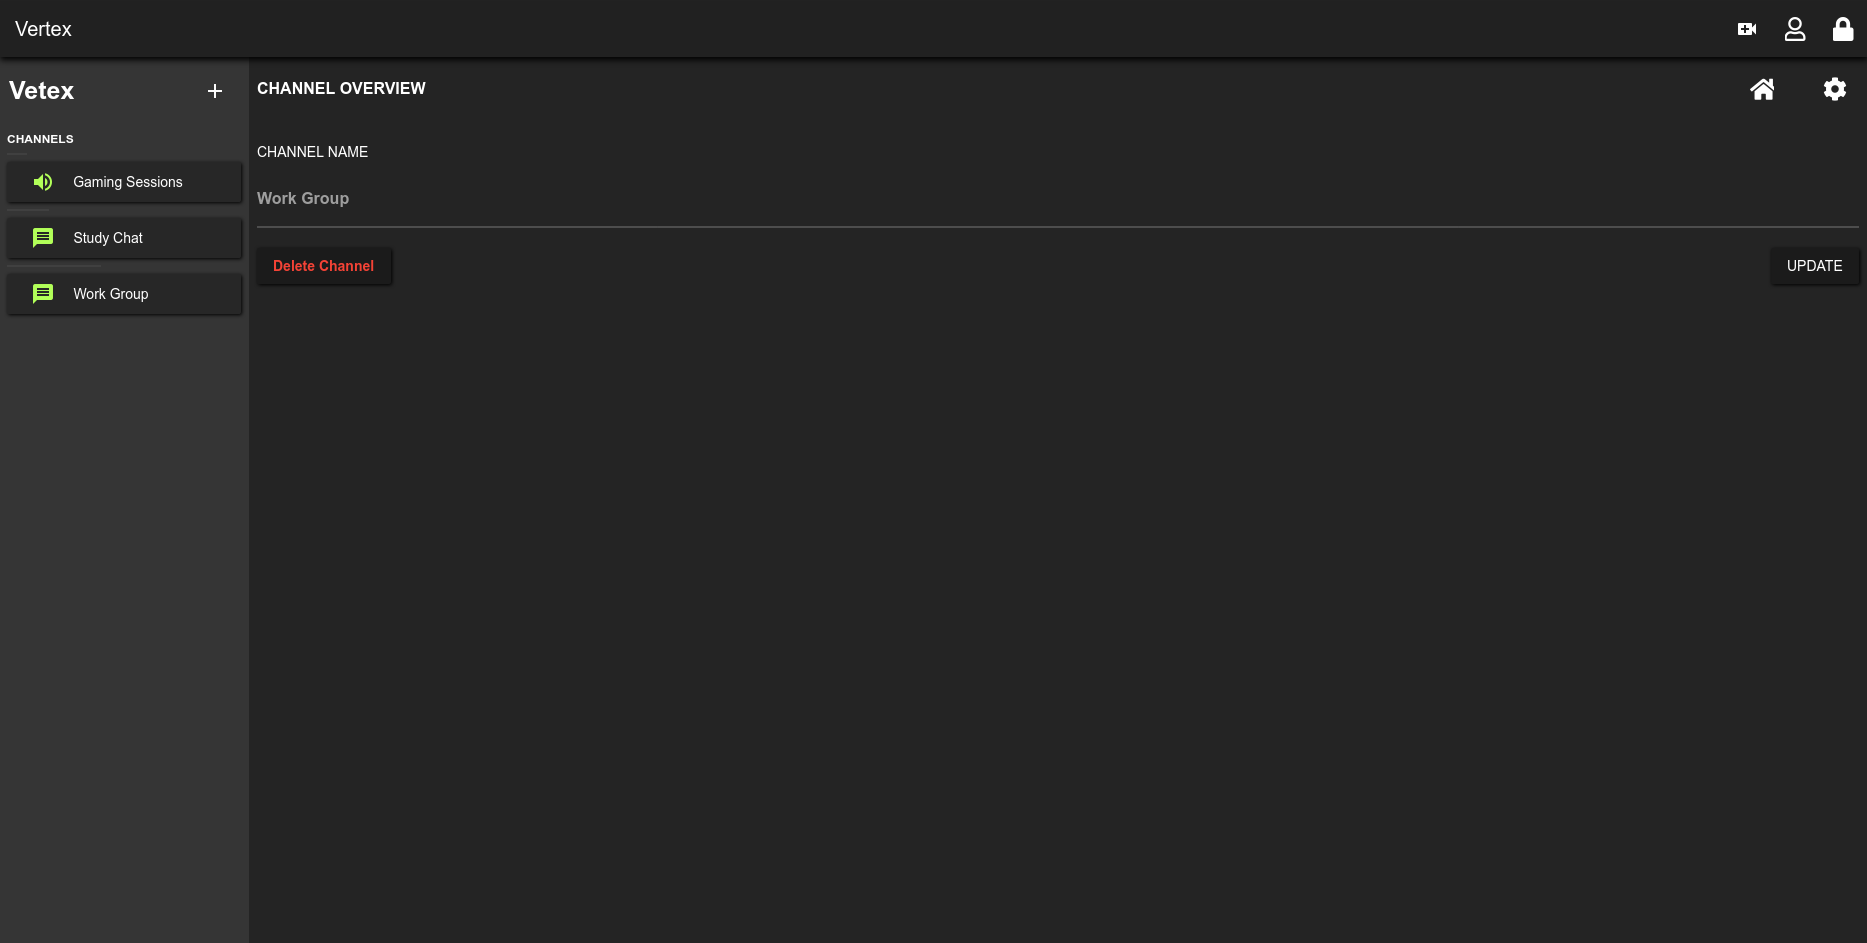
\includegraphics[width=0.7\textwidth]{images/pageScreenshots/channelDeletion.png}
\end{figure}

Settings Page See Figure ~\ref{image:settingsPage}
\begin{figure}[h!]
    \caption{Settings Page}
    \label{image:settingsPage}
    \centering
    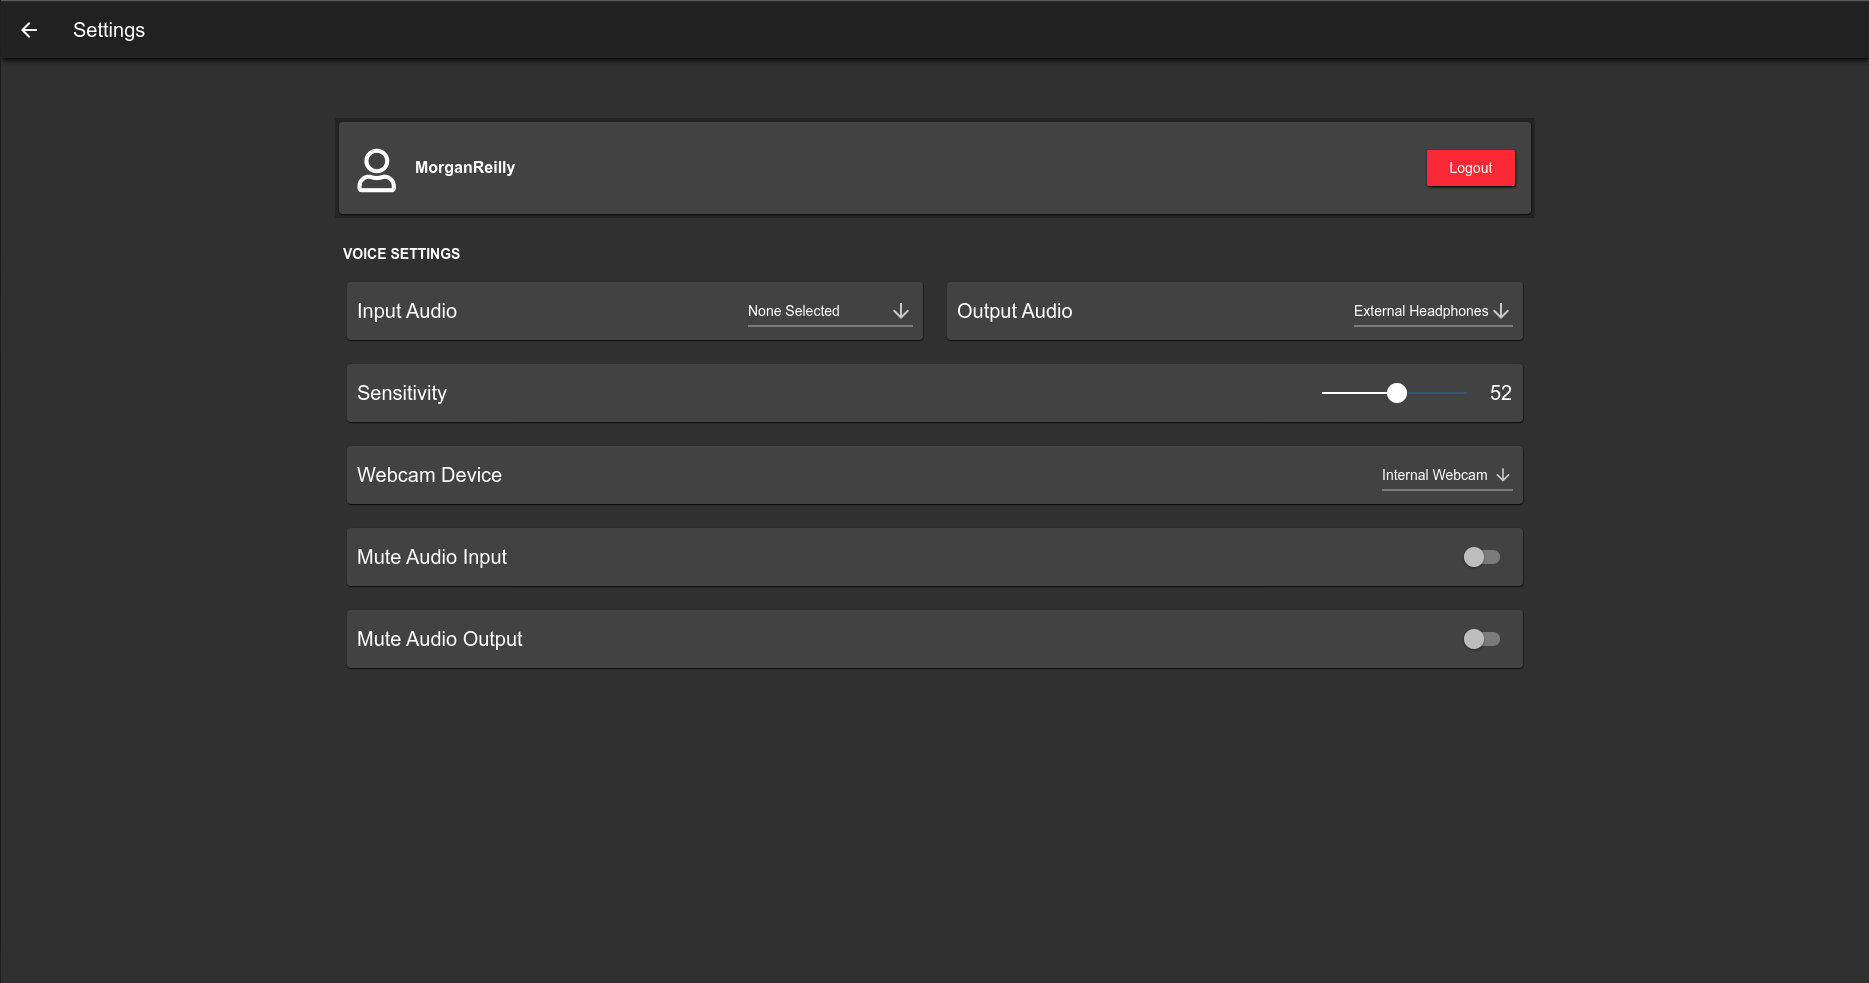
\includegraphics[width=0.7\textwidth]{images/pageScreenshots/settingsPage.png}
\end{figure}


\section{Database}
For vertex a MySQL was chosen as the application database. This was ultimately a big decision as the application could have used any assortment of SQL style databases, a noSQL database, or could have gone with a graph database, or possibly even a document store.
\\ This database uses an INNODB engine, which allows for full transaction support, various levels of locking, such as row-locking, and has full ACID compliance. The alternative which could have been used is a MYISAM engine, which supports different functionality which would not have suited the application.

\subsection{Schemas}
Due to the nature of the application only a handful of schemas were needed to handle the information saved throughout the application. The information being held is relatively straightforward. For each of the tables they need a unique identifier. In the case of schemas: User; Channel; Message; and Session; this was handled with the use of an auto-incrementing integer value, which increments by 1 per entry and starts at various values in respect to each table i.e. User will auto-increment from 100, Channel will auto-increment from 200 and so on. These auto-incrementing values are used in the form of the primary key for those tables with an alias of ‘id’ for each table allow for an ease of lookup, along with an O(1) time-complexity for look-up.
\\ The other remaining table, Member, uses foreign key values in a unique combination to handle look up, instead of a primary key value. For the most part, since there are few components of entry in each schema, the varaibles are given a ‘NOT NULL’ modifier, which means that data has to be given to them in order to avoid errors being raised.
\\ The database uses UTF-8 default as it’s character set, and utf8\_general\_ci as it’s collate set.
\\ The following schemas use cascading update, and cascading delete: Channel; Message; Session; Member. This allows for safe removal or modification of data, without setting null values.

\subsubsection{User Schema}
This schema handles the user information and was the first schema which had to be thought about.
\\ The User table is broken down into 3 components: ‘id’, ‘name’, ‘password’.
\\The ‘id’ of this table is described above, as an unsigned auto-incrementing integer starting at 100.
\\The ‘name’ is stored as a varchar of size 32 with a not-null modifier. This allows for an adequate size of allocated storage for the user name. The purpose of limiting the character is for memory preservation. The ‘name’ acts as a unique key to this schema. This is to avoid any duplication errors for any new users being inputted into the table, and also serves as a reference point should the ‘name’ need to be queried without explicitly knowing the ‘id’ beforehand. 
\\The ‘password’ is stored after it is hashed and salted using the bcrypt hashing function, which utilises the blowfish cipher. It is stored as a varchar of size 255 with a not null modifier.
See Figure ~\ref{image:userSchema}

\subsubsection{Channel Schema}
This schema handles the channels being used in the application, and is broken down into 4 components.
\\The ‘id’ of this table is described above, as an unsigned auto-incrementing integer starting at 200.
The channel has to store a ‘name’ which forms part of a unique key used for referencing and duplication avoidance. This value is stored as a varchar of size 32 with a not null modifier.
\\It has a 'creator\_id', which acts as a foreign key from the User table (id).
\\It has a enumerated value, ‘type’, which allows us to differentiate between voice and text channels. This allows the user to create channels with a bit of variance to them.
\\Its unique key consists of ‘name’, ‘creator\_id’, and ‘type’ which serves as a way to avoid duplication's in the database.
See Figure ~\ref{image:channelSchema}

\subsubsection{Message Schema}
This schema handles the messages being sent in the application. It is broken down into 5 components.
\\The first being the ‘id’. This is an unsigned auto-incrementing integer starting at 300.
\\The second being ‘channel’, which is a foreign key relating to the Channel table (see Channel for details). This serves as a way to link the message to the channel, without the messages spilling out into incorrect channels.
\\The third component is the ‘author’, which is a foreign key relating to the User table (see User for details). It serves as a way to link the message to the relevant user, without incorrect users seeing the data.
The fourth component is ‘content’. This is a varchar of size 255 with a not null modifier. This variable stores the message content that the user is sending.
\\The final component of this schema is the ‘timestamp’ for the message. This is stored as an Int of size 8 with a not null modifier.  The timestamp is stored as Unix Epoch time and the purpose of the size being set to 8 for this is to allocate enough space to handle epoch time correctly.
See Figure ~\ref{image:messageSchema}

\subsubsection{Session Schema}
This schema handles the current session that is active for the user. It is a fairly straight-forward schema which consists of 3 components.
\\ The first component is the ‘id’. This is a varchar of size 255 with a not null modifier. The reason being is that the id should be stored as a UUID, therefore requiring an adequate amount of space allocation for the variable. This is the primary key for this table.
\\ The second component is ‘user’. This is a foreign key which links this table to the User table (see User for details).
The final component is ‘expire\_after’. This is another instance of Unix Epoch time, with a similar allocation of memory for this variable as was seen in the Message table. 
See Figure ~\ref{image:sessionSchema}

\subsubsection{Member Schema}
The final table in this database is the Member table. This is responsible for grouping users with relevant channels, which allows for easier look-ups. It consists of 2 components, both of which are foreign keys.
\\ The first component is ‘channel’. This is set as an Integer of size 4, and is a  foreign key which relates to the Channel table on ‘id’.
\\ The second, and final component, is the ‘user’. This is also set as an Integer of size 4, and is a foreign key which relates to the User table on ‘id’.
\\ This table contains a unique key, which is comprised of  ‘channel’ and ‘user’. The reason being is to avoid duplicate entries in this schema, and also helps with look ups on the table.
See Figure ~\ref{image:memberSchema}

\subsection{Testing}
In terms of testing, a full CRUD test is included in ‘vertex\_db\_v2.sql’, which is located on the database portion of the project repository. These tests verify correct functionality of creation of values, reading values, updating values, and deletion of values. They also verify and test for referential integrity for the database, along with duplication avoidance.

\begin{figure}[h!]
    \caption{User Schema}
    \label{image:userSchema}
    \centering
    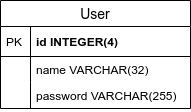
\includegraphics[width=0.3\textwidth]{images/UserSchema.png}
\end{figure}

\begin{figure}[h!]
    \caption{Channel Schema}
    \label{image:channelSchema}
    \centering
    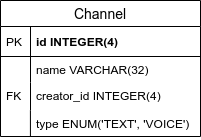
\includegraphics[width=0.3\textwidth]{images/ChannelSchema.png}
\end{figure}

\begin{figure}[h!]
    \caption{Message Schema}
    \label{image:messageSchema}
    \centering
    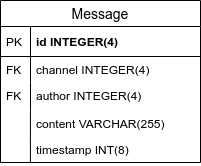
\includegraphics[width=0.3\textwidth]{images/MessageSchema.png}
\end{figure}

\begin{figure}[h!]
    \caption{Session Schema}
    \label{image:sessionSchema}
    \centering
    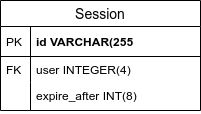
\includegraphics[width=0.3\textwidth]{images/SessionSchema.png}
\end{figure}

\begin{figure}[h!]
    \caption{Member Schema}
    \label{image:memberSchema}
    \centering
    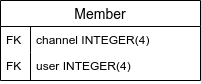
\includegraphics[width=0.3\textwidth]{images/MemberSchema.png}
\end{figure}

\begin{figure}[h!]
    \caption{Database Schema}
    \label{image:databaseSchema}
    \centering
    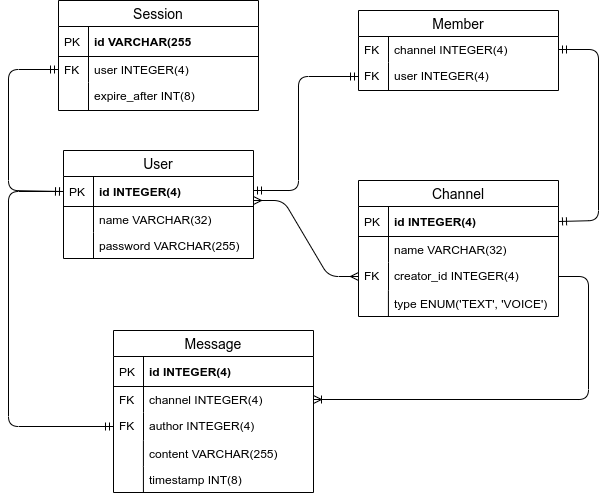
\includegraphics[width=1\textwidth]{images/FullSchemaDesign.png}
\end{figure}